\chapter{\IfLanguageName{dutch}{Stand van zaken}{State of the art}}%
\label{ch:stand-van-zaken}

\section{Inleiding}

Het onderzoek start met een uitgebreide literatuurstudie over de benodige kennis binnen het logopedisch, taal- en informatica vakdomein om geautomatiseerde en gepersonaliseerde vereenvoudigdigde teksten te verkrijgen van wetenschappelijke artikelen. Om een toepassing voor gepersonaliseerde en geautomatiseerde tekstvereenvoudiging van wetenschappelijke artikelen  op maat van deze doelgroep aan te reiken, is het van cruciaal belang om de noden van scholieren met dyslexie in de derde graad van het middelbaar onderwijs te benoemen. Het onderzoek benoemt bewezen noden met behulp van een literatuurstudie. Daarnaast kaart het de huidige problemen bij wetenschappelijke artikelen aan. Wetenschappelijke artikelen vereenvoudigen op maat voor scholieren met dyslexie kan volgens taalexperten op verschillende manieren. Het is belangrijk om stil te staan bij de bestaande en reeds bewezen handmatige tekstvereenvoudigingstechnieken. Vervolgens komen technieken voor geautomatiseerde tekstvereenvoudiging (ATV) aan bod. Zowel de nodige informatie van taalverwerking met AI, als de huidige AI-technologieën voor tekstvereenvoudiging zijn gegeven. Ten slotte zijn AI- technologieën hoogstaand en ontwikkelaars maken deze alsmaar robuuster, maar het is cruciaal om bij dit onderzoek aandacht te besteden aan de mogelijke problemen die AI- ontwikkelaars moeten vermijden of waarvan zij zichzelf attent op moeten maken. 

\section{Specifieke noden en richtpunten}

Om wetenschappelijke artikelen te vereenvoudigen op maat van de unieke noden van scholieren met dyslexie moet het onderzoek stilstaan bij de specifieke noden van scholieren met dyslexie in de derde graad van het middelbaar onderwijs, alsook bij de moeilijkheden bij het begrijpend lezen van wetenschappelijke artikelen. Deze sectie bespreekt eerst algemeen hoe scholieren met dyslexie bij het begrijpend lezen kunnen worden geholpen. Daarna worden de belemmeringen en moeilijkheden van wetenschappelijke artikelen aangekaart. Deze sectie beantwoordt de volgende twee onderzoeksvragen: 

\begin{itemize}
	\item Welke specifieke noden hebben scholieren met dyslexie van de derde graad middelbaar onderwijs bij het begrijpen van complexere teksten?
	\item Wat zijn de specifieke kenmerken van wetenschappelijke artikelen?
\end{itemize}

\subsection{Specifieke noden van scholieren met dyslexie in de derde graad van het middelbaar onderwijs.}

Leesvaardigheid is geen aangeboren vaardigheid, maar iets dat mensen zelf moeten aanleren \autocite{Bonte2020, VanDerMeer2022}. Hoewel dit proces vlot kan verlopen, kunnen mensen met dyslexie benadeeld worden tijdens dit proces.  Dyslexie wordt gekenmerkt door beperkt lezen en kan het voorlezen traag, radend en letter-voor-letter maken. Mensen met dyslexie kunnen tijdens het begrijpend lezen verschillende drempels ervaren; die worden in tabel \ref{table:dyslexia-hurdles} opgesomd.

\begin{center}
	\begin{table}[H]
	\begin{tabular}{ | m{9cm} | m{6cm} | } 
		\hline
		\textbf{Kenmerk} & \textbf{Bron} \\ 
		\hline
		Trage woordbenoeming &  \autocite{Bonte2020} \\
		\hline
		Problemen bij het leesbegrip & \autocite{Gala2016, Bonte2020} \\ 
		\hline
		Hardnekkig letter-voor-letter lezen & \autocite{Bonte2020, Zhang2021} \\ 
		\hline
		Problemen met woordherkenning en -herinnering & \autocite{Bonte2020} \\
		\hline
		Moeite bij homofonische of pseudo-homofonische woordenschat & \autocite{Zhang2021} \\
		\hline
		Moeite bij onregelmatige lettergreepcombinaties & \textcite{Gala2016} \\
		\hline
	\end{tabular}
	\caption{Specifieke drempels bij het begrijpend lezen van een tekst.}
	\label{table:dyslexia-hurdles}
	\end{table}
\end{center}

\medspace

De digitalisering evolueerde de voorbije twintig jaar in stijgende lijn en scholieren in de tweede en derde graad zijn, door het gebruik van smartphones en laptops, hier het meeste vatbaar bij zowel thuisgebruik als gebruik in het onderwijs. Verder omschrijft dit artikel een checklist van technische elementen waaraan een webpagina of toepassing moet voldoen om een leesbare ervaring te voorzien voor scholieren met dyslexie. Tabel \ref{table:dyslexia-necessaries} geeft deze noden weer.

\begin{center}
		\begin{table}[H]
	\begin{tabular}{ | m{8cm} | m{7cm} | } 
		\hline
		Kenmerk & Bron \\
		\hline
		Zachtgele, -groene -of bruine ahtergrondkleur 	& \textcite{Santana2012} \\ \hline
		Lettergrootte vergroten naar 14pt 				& \autocite{Rello2015} \\ \hline
		Woord- en karakterspatiëring 					& \textcite{Santana2012, Rello2013b} \\ \hline
		Consistente lay-out 							& \autocite{Rello2015} \\  \hline
		Waarschuwingen geven omtrent formulieren, sessies (login) & \\ \hline
		Consistente lay-out 							& \autocite{Rello2015, Fernando2021} \\ \hline
		Duidelijk zichtbare koppen- of headingstructuur & \autocite{Rello2012a} \\ \hline
		Duidelijke symbolen gebruiken 					& \autocite{Rello2013b} \\ \hline
		Inhoud visueel groeperen 						& \autocite{Rello2015, Fernando2021}\\ \hline
		Huidige positie benadrukken 					& \autocite{Fernando2021} \\ \hline
		
	\end{tabular}
	\caption{Oplossingen die software-ontwikkelaars kunnen aanreiken bij een toepassing of website.}
	\label{table:dyslexia-necessaries}
	\end{table}
\end{center}

\subsection{Specifieke kenmerken van wetenschappelijke artikelen}

Wetenschappelijke artikelen zijn van cruciaal belang voor het verspreiden van nieuwe kennis en onderzoeksresultaten, maar toch blijven ze voor velen een mysterieus en ontoegankelijk gebied vanwege de complexiteit van de inhoud en het technische jargon dat onmisbaar lijkt te zijn \autocite{Ball2017}. Dit kan het begrip van de artikelen bemoeilijken, vooral bij begrijpend lezen, en vormt daarmee een extra obstakel bij het gebruik van wetenschappelijke artikelen als bron van kennis tijdens de les. Wetenschappelijke artikelen volgen IMRAD, een uniform formaat voor gepubliceerde wetenschappelijke artikelen, dat bestaat uit vijf hoofdstukken: samenvatting, inleiding, methodologie, resultaten en discussie. Hoewel het middelbaar en hoger onderwijs deze artikelen gebruiken als leermiddel,  is  de inhoud van een hoger niveau en voornamelijk gericht op mensen uit het vakgebied. \textcite{Pain2016, CAS2021} benadrukken de complexiteit van wetenschappelijke artikelen en de volgende aspecten waarom ze moeilijk te interpreteren zijn.

\medspace

Tabel \ref{table:scientific-paper-struggles} somt deze factoren op. Hoewel wetenschappelijke artikelen over een grote drempel bezitten, betrekken ze jongeren met wetenschappelijk onderzoek, alsook leren ze een discussieerbaar en kritische vaardigheid. 

\medspace

\begin{center}
	\begin{table}[H]
	\begin{tabular}{| m{5cm} | m{10cm} |}
		\hline
		\textbf{Probleem} & \textbf{Oplossing} \\
		\hline
		Veel informatie in een compact formaat of \textit{high information density} & Extra uitleg schrijven bij compacte zinnen, zoals extra uitleg bij woorden of zinnen herschrijven. \\
		\hline
		Hoog gebruik van meerlettergrepige woorden & Eenvoudigere synoniemen gebruiken. \\
		\hline
		Wetenschappelijk jargon & Rekening houden met een doelgroep buiten het vakgebied door eenvoudigere synoniemen te schrijven. Indien deze niet beschikbaar zijn, kan er extra uitleg als alternatief worden gegeven. \\
		\hline
		Complexe concepten & Paragrafen herschrijven zodat ze eerst uitleg geven op een high-level niveau. Vervolgens lagen van complexiteit toevoegen om de lezer te begeleiden doorheen de methodologie, discussie en conclusie van het wetenschappelijk artikel. \\ 
		\hline
		Cijfermateriaal bij resultaten & De interpretatie van percentages of cijfermateriaal schrijven. Zoals 'ongeveer een kwart van de bevolking' in plaats van '24.97\% van de bevolking'. \\
		\hline
	\end{tabular}
	\caption{Complexe leesfactoren van een wetenschappelijk artikel.}
	\label{table:scientific-paper-struggles}
	\end{table}
\end{center}

Scholieren met verschillende achtergronden verschillen vaak in achtergrondkennis, wat invloed kan hebben op het tekstbegrip \autocite{DeMeyer2019}. Zo kunnen scholieren met een achtergrond in fysica sneller de draad oppikken bij het lezen van fysica-gerelateerde artikelen dan scholieren met een economische achtergrond. Dit maakt het moeilijk om de leesbaarheid van een tekst objectief te beoordelen. Het jargon kan voor de ene groep scholieren makkelijk zijn, en voor de andere groep moeilijk.

\medspace

Onderzoeken en ontwikkelaars zorgden voor de geautomatiseerde berekening van leesmetrieken. Dankzij Python-libraries, zoals Textstat\footnote{textstat} en Readability\footnote{https://pypi.org/project/readability/}, kunnen ontwikkelaars via commandline-toepassingen deze processen om leesmetrieken te berekenen automatiseren. Zo zijn drie prevalente leesbaarheidsscores weergegeven in tabel \ref{table:readability-scores}. Daarnaast kunnen toepassingen, zoals Textinspector\footnote{https://textinspector.com/}, analytisch inzicht geven in de complexiteit van Engelstalige teksten. Er bestaat echter geen alternatief dat leesgraadsscores kan berekenen voor Nederlandstalige wetenschappelijke artikelen. Het is wel belangrijk om te benadrukken dat deze leesbaarheidsscores geen rekening houden met de achtergrondkennis van mogelijke lezers.

\begin{center}
	\begin{table}[H]
	\begin{tabular}{ | m{5cm} | m{10cm} | } 
		\hline
		\textbf{Score} & \textbf{Uitleg} \\ 
		\hline
		Flesch Reading Ease (FRE) & Deze leesbaarheidsscore berekent de moeilijkheidsgraad op zinsbasis. Hoe hoger de score, hoe 'eenvoudiger' de zin. \\
		\hline
		Gunning FOG (FOG) & In tegenstelling tot FRE, berekent FOG de moeilijkheidsgraad op basis van de volledige tekst. \\
		\hline
		Complexe woorden volgens \textit{Dale-Chall Index} (DCI) & Deze lijst omvat woorden die experimenten bij Amerikaanse tieners als complex omschrijven. De DCI werkt per leeftijdscategorie. \\
		\hline
	\end{tabular}
	\caption{Prevalente leesgraadsscores.}
	\label{table:readability-scores}
	\end{table}
\end{center}

Diverse onderzoeken van de afgelopen tien jaar wijzen uit dat wetenschappelijke teksten steeds complexer worden. Dat maakt deze teksten voor niet-experten en niet-doctoraatsstudenten minder toegankelijk, vanwege het gebruik van technisch jargon en ingewikkelde zinsstructuren \autocite{Ball2017, PlavenSigray2017, Jones2019}. Deze trend begon volgens onderzoek al in de tweede helft van de twintigste eeuw \autocite{Hayes1992}.

\medspace

Volgens onderzoek van \textcite{PlavenSigray2017} is de taal van wetenschappelijke artikelen de laatste jaren steeds complexer geworden. Uit een vergelijkende studie tussen abstracts en de rest van de inhoud van wetenschappelijke tijdschriften blijkt dat abstracts het meest complexe deel van een artikel vormen. De evolutie van de leesbaarheid wordt weergegeven in figuur \ref{img:fre-ndc}, dat ook de FRE- en NDC-scores toont. Het onderzoek schat dat 22\% van alle wetenschappelijke artikelen op het niveau van een masterstudent in het Engels geschreven zijn, tegenover 14\% in 1960. Deze trend is belangrijk om op te volgen in de komende decennia, omdat het een obstakel kan vormen voor toekomstige generaties.

\begin{figure}[H]
	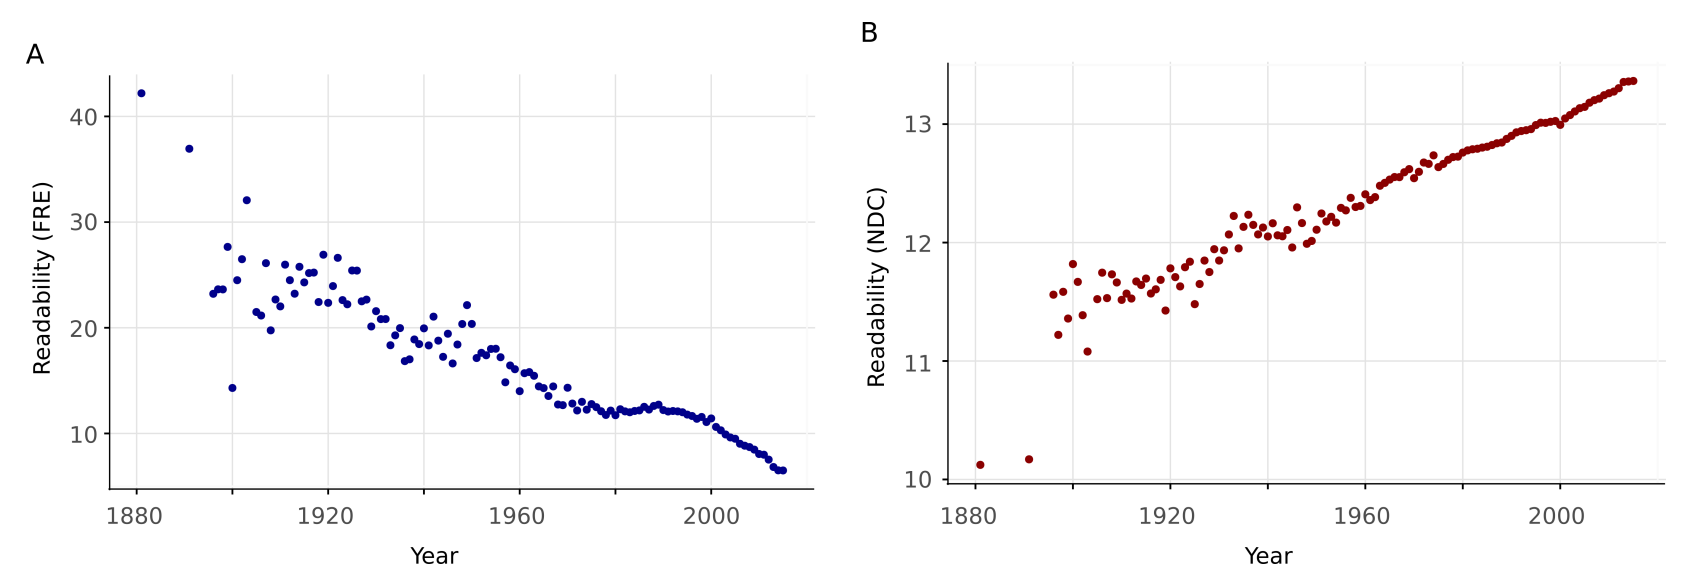
\includegraphics[width=\linewidth]{img/fre-ndc.png}
	\caption{De toename van vereiste leesgraad volgens FRE (links) en NDC (rechts). Bron: \autocite{PlavenSigray2017}}
	\label{img:fre-ndc}
\end{figure}

Onbegrijpelijke en ontoegankelijke zinsstructuren hinderen ook vakexperten. Zo toonde onderzoek van \textcite{McNutt2014} aan dat begrip van de methodologie en resultaten cruciaal is in het kader van reproduceerbaarheid; enkel zo kunnen wetenschappers op correcte wijze een studie reproduceren en wetenschappelijke inzichten bevestigen of met verdere resultaten verrijken. Experimenten van \textcite{Hubbard2017} wijzen namelijk uit dat het net vooral de methodologie en resultaten van een wetenschappelijk artikel zijn die een hoge leesgraad vergen. In deze context is ook het onderzoek van \textcite{Hartley1999} en \textcite{Snow2010} relevant waarin ze aantonen dat het herschrijven van abstracts de begrijpbaarheid ervan kan verhogen.

\medspace

Volgens \textcite{Hollenkamp2020, McCombes2022} moeten vereenvoudigde of samengevatte wetenschappelijke artikelen drie vragen kunnen beantwoorden: waarom werd het onderzoek uitgevoerd, wat zijn de experimenten en wat zijn de conclusies van de onderzoekers? Dit omvat de achtergrondinformatie, hypotheses, methoden, resultaten, implicaties, beperkingen en aanbevelingen. De tekst omzetten in een ander formaat zoals post-it notes, tabelvorm of opsommingen, maakt het beter begrijpbaar \autocite{Rijkhoff2022}. 

\medspace

Wetenschappelijke artikelen zijn voornamelijk in PDF-formaat terug te vinden. Dit formaat valt eenvoudig in te lezen met Python-pakketten, waaronder PDFMiner of PyPDF. Wel ondervinden ontwikkelaars soms problemen bij het in- lezen van PDF-bestanden: niet alle tekst of kan uit de PDF worden geëxtraheerd. Als oplossing kunnen ontwikkelaars gebruik maken van \textit{optical character recognition} of OCR. In Python zijn er pakketten die deze technologie eenvoudig kunnen realiseren, namelijk EasyOCR en Tesserat.

\section{Aanpakken voor tekstvereenvoudiging}
% Welke aanpakken zijn er voor geautomatiseerde tekstvereenvoudiging? 

\subsection{Manuele tekstvereenvoudiging}
% Hoe worden teksten handmatig vereenvoudigd voor scholieren met dyslexie? 

Voor sommige lezers kan het begrijpend lezen van een complexe tekst echter een uitdaging zijn, zoals scholieren met dyslexie. \textit{Manual tekst simplification} of MTS kan deze groep helpen \autocite{Siddharthan2014}. De techniek van MTS gebruikt eenvoudige woordenschat en zinsstructuren en maakt structurele aanpassingen om de tekst vlotter leesbaar te maken. MTS is het proces dat het technische leesniveau en het woordgebruik van een geschreven tekst vermindert. Dit leidt tot een betere leeservaring zonder het verlies van de kerninhoud tijdens het lezen van de tekst.

\begin{center}
		\begin{table}[H]
			\begin{tabular}{ | m{4cm} | m{8cm} | m{3cm} | } 
			\hline
			Type vereenvoudiging & Techniek & Bron \\ \hline
			
			LS & Moeilijke woorden vervangen door eenvoudigere synoniemen & \autocite{Rello2013c, Siddharthan2014} \\ 
				& Woorden- en synoniemenlijst maken & \\
				& Dubbelzinnige woorden vervangen & \\
				& Idiomen vervangen & \\ 
				& Rekening houden met het gekende jargon van de doelgroep &\\
			\hline
			SS & Tangconstructies aanpassen &\\
			& Zinnen langer dan negen woorden inkorten &\\
			& Verwijswoorden aanpassen &\\
			& Voorzetseluitdrukkingen aanpassen &\\
			& Samengestelde werkwoorden aanpassen &\\
			& Actieve stem gebruiken & \autocite{Ruelas2020} \\
			& Onregelmatige werkwoorden vermijden &\\
			\hline
			Structurele aanpassingen & Marges aanpassen &\\
			& Lettertype en -grootte aanpassen &\\
			& Woord- en karakterspatiëring aanpassen &\\
			& Herschrijven en -structureren als opsomming of tabelvorm &\\
			\hline
		\end{tabular}
		\caption{Drie algemene technieken voor MTS.}
		\label{table:manual-simplification}
	\end{table}
\end{center}

\subsection{Bevoordelende effecten van MTS bij scholieren met dyslexie}

Onderzoek toont aan dat vereenvoudigde teksten het leesbegrip en woordherkenning van kinderen met dyslexie significant kunnen verbeteren \autocite{RiveroContreras2021}. Bovendien blijkt uit experimenten dat frequent woordgebruik de ontcijfertijd bij mensen met dyslexie significant vermindert, en dat teksten met verminderde lexicale complexiteit minder leesfouten opleveren voor mensen met dyslexie \autocite{Rello2013a, Gala2016}. Deze studies benadrukken ook moeilijkheden van kinderen met dyslexie bij het lezen van woorden met onregelmatige lettergreepcombinaties. Mensen zonder dyslexie bereiken doelwaarden onder optimale omstandigheden, zoals aangegeven door de richting van de pijl op figuur \ref{img:readability-mean-fixation-duration}. Het gebruik van veelvoorkomende woorden vermindert de decodeertijd en verbetert het leesbegrip voor mensen met dyslexie.

\medspace

\begin{figure}
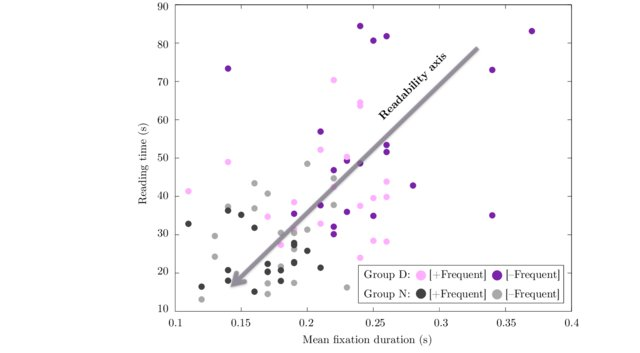
\includegraphics[width=\linewidth]{img/readability-mean-fixation-duration.png}
\caption{De gemeten \textit{mean fixation duration} tijdens begrijpend lezen uit het onderzoek van \textcite{Rello2013a}.}
\label{img:readability-mean-fixation-duration}
\end{figure}

\medspace

Hoewel onderzoeken de positieve effecten van lexicale vereenvouding voor lezers met dyslexie onderstrepen, is er relatief weinig onderzoek gedaan naar de effecten van syntactische vereenvoudiging op kinderen en scholieren met dyslexie. In het experiment van \textcite{Linderholm2000} had het aanpassen van causale structuren een significant effect op het leesbegrip en de foutenmarge van de bevraagden met een lage leesgraad. Door coherentieonderbrekingen te herstellen en tekstgebeurtenissen in een tijdsafhankelijke volgorde te plaatsen, konden zowel vaardige als minder vaardige lezers profiteren van de revisies. Verbaal parafraseren had geen significant effect op lezers met dyslexie, volgens \textcite{Rello2013c}. De bevraagden waren tussen de 13 en 37 jaar oud, met een gemiddelde leeftijd van 21 jaar. Het tekstformaat bleef ongewijzigd, maar lettertypes werden aangepast.

\medspace

Het onderzoek van \textcite{Nandhini2013} experimenteerde met een andere vorm van aanpassingen om de leesbaarheid van teksten te verhogen, namelijk gepersonaliseerde samenvattingen. Het experiment in het onderzoek maakt gebruik van onaangepaste zinnen uit de oorspronkelijke tekst die op maat van de lezer zijn gepresenteerd en herstructureert deze volgens de oorspronkelijke tekst. Door de belangrijkste zinnen onaangepast te laten en de structuur aan te passen, is de tekst toegankelijker voor de lezer. Hoewel de onderzoekers de rusulterende logische structuur in twijfel trokken, was de leesbaarheid van teksten bij de deelnemers significant beter dan bij de oorspronkelijke tekst, zonder negatieve effecten op het leesbegrip.

\medspace

Tot slot hebben onderzoeken aangetoond dat scholieren met dyslexie gevoeliger zijn voor veranderingen in visuele parameters, zoals lettertype, karakterafstand, tekst- en achtergrondkleur en grijswaarden. Minimalistische ontwerpen met pictogrammen behoren tot de aanbeveling om de leesbaarheid te verbeteren, evanals lettergrootte groter dan 14pt en een \textit{sans-serif}, \textit{monospaced} of \textit{roman} lettertype. Volgens \textcite{Rello2015, Bezem2016, Rello2017} zijn lichtgrijze achtergronden met zwart lettertype op een gele achtergrond, of zachtgele, -groene of lichtblauwe achtergrondkleuren de beste kleurencombinaties. Het gebruik van lettertypen zoals OpenDys heeft geen effect op lezers met of zonder dyslexie, terwijl cursieve lettertypen worden afgeraden, aldus \textcite{Rello2013b, Rello2015}.

\medspace

Tabel \ref{table:benefits-mts} somt de bewezen strategieën op samen met de bewezen voordelen tijdens het begrijpend lezen.

\medspace

\begin{center}
	\begin{table}[H]
	\begin{tabular}{ | m{5cm} | m{5cm} | m{5cm} | } 
	\hline
	\textbf{Techniek} & \textbf{Bewezen voordeel} & \textbf{Bron}\\
	\hline
	Frequent woordgebruik & Lagere decodeertijd & \\
	& Beter leesbegrip & \\
	\hline	
	Verwerpen van onregelmatige lettergrepen & Verminderde decodeertijd & \\
	& Beter leesbegrip & \\	
	\hline
	Causale structuren aanpassen & Beter leesbegrip &\\
	& Minder fouten bij het begrijpend lezen & \\
	\hline	
	Tekstgebeurtenissen in een tijdsafhankelijke volgorde plaatsen & Beter leesbegrip bij het reviseren & \\
	\hline
	Coherentieonderbrekingen herstellen & Beter leesbegrip bij het reviseren & \\
	\hline
	Gepersonaliseerde samenvatting & Betere leesbaarheid & \\
	\hline
	Zachtkleurige achtergrond & Betere leesbaarheid & \\
	\hline
	Niet-cursieve, sans-serif lettertypen & Betere leesbaarheid & \\
	\hline 
	Lettertype groter dan 14pt & Betere leesbaarheid & \\
	\hline
	\end{tabular}
	\caption{Bewezen voordelen van MTS op mensen met dyslexie tijdens het begrijpend lezen.}
	\label{table:benefits-mts}
	\end{table}
\end{center}

\subsection{Aanpak voor ATS.}
% Welke toepassingen, tools en modellen zijn er beschikbaar om Nederlandse geautomatiseerde tekstvereenvoudiging met AI mogelijk te maken? 

De laatste evolutie in machinaal leren biedt een mogelijkheid om dit proces te automatiseren. \textit{Automatic text simplification} of ATS is een onderdeel van natuurlijke taalverwerking binnen machinaal leren (ML). Dit omvat technieken zoals tekstanalyse, taalherkenning, -generatie, spraakherkenning en -synthese, en semantische analyse. NLP stelt computers in staat om menselijke taal te begrijpen en te communiceren op een natuurlijke manier. De begrippen die volgen worden behandeld in \textcite{Sohom2019, Eisenstein2019} en zijn cruciaal voor de daaropvolgende concepten.

\medspace

Zo dient tokenisatie om zinnen op basis van tokens te splitsen. Er zijn vier manieren om tokens in een tekst te splitsen en zo een woordenschat op te bouwen, namelijk op woord-, karakter-, subwoord- en zinniveau, volgens onderzoek van \textcite{Menzli2023}. Bij karaktertokenisatie neemt de inputlengte toe, maar dit heeft volgens \textcite{Ribeiro2018} weinig bruikbare \textit{use cases}. Het opsplitsen van zeldzame woorden in kleinere stukken om een woordenschat op te bouwen biedt voordelen ten opzichte van woordtokenisatie, aldus \autocite{Iredale2022}.

\medspace

In NLP is het lemmatiseren gebaseerd op \textit{stemming}, ofwel een NLP-taak waarbij de stam van een woord wordt genomen, maar het houdt ook rekening met de betekenis van elk woord. Er zijn Nederlandstalige modellen beschikbaar voor lemmatiseren, zoals JohnSnow\footnote{https://nlp.johnsnowlabs.com/2020/05/03/lemma\_nl.html}. Bij omgekeerd lemmatiseren wordt een afgeleide van de stam bepaald, bijvoorbeeld enkelvoud of meervoud voor zelfstandige naamwoorden zoals 'hond' \autocite{Eisenstein2019}. Bij het \textit{parsen} krijgt elk woord of zinsdeel een label toegewezen, zoals zelfstandig naamwoord, bijwoord, werkwoord, bijzin of stopwoord. Het identificeren van zinsdelen wordt \textit{chunking} genoemd. \textit{Parsing} is vatbaar op ambiguïteit, omdat bijvoorbeeld een 'plant' niet gelijk is aan de vervoeging van het werkwoord 'planten' \autocite{Eisenstein2019}.

\medspace

In NLP baseert het lemmatiseren zich op stemming, een NLP-taak waarbij deze de stam van een woord neemt, maar ook rekening houdt met de betekenis van elk woord. Er zijn Nederlandstalige modellen beschikbaar voor lemmatiseren, zoals JohnSnow⁴. Omgekeerd lemmatiseren werkt door een afgeleide vorm van de stam te bepalen, bijvoorbeeld enkelvoud of meervoud voor zelfstandige naamwoorden als ’hond’ \autocite{Eisenstein2019}. Bij het parsen krijgt elk woord of zinsdeel een label toegewezen, zoals zelfstandig naamwoord, bijwoord, werkwoord, bijzin of stopwoord. De identificatie van zinsdelen heet chunking. Parsing is vatbaar op ambiguïteit omdat bijvoorbeeld ‘een plant’ niet gelijk is aan de vervoeging van het werkwoord ’planten’ \autocite{Eisenstein2019}.

\medspace

Om de betekenis van elk woord in een tekst te begrijpen, moet een machine in staat zijn om de betekenis achter elk token te begrijpen. Dit is waar \textit{sequence labeling} om de hoek komt kijken, volgens \textcite{Eisenstein2019}. Elk woord in een tekst krijgt een label voor \textit{Part-of-Speech} (PoS) of \textit{Named-Entity-Recognition} (NER). Deze fase van NLP achterhaalt de structuur van een tekst. PoS-tagging richt zich op de grammaticale categorieën van woorden, terwijl NER-labeling zich richt op het herkennen van specifieke entiteiten in een tekst. Bij PoS-tagging worden de woorden in een zin geanalyseerd. Elk woord krijgt een koppeling aan een grammaticale categorie, zoals een zelfstandig naamwoord, werkwoord, bijvoeglijk naamwoord of bijwoord. \textit{PoS-tagging} helpt bij het begrijpen van de syntactische structuur van een zin en is nuttig bij parsing en machinevertaling. Een voorbeeld van PoS-tagging is te zien in figuur \ref{fig:pos-labeling} en is afkomstig uit \textcite{Bilisci2021}.

\begin{center}
	\begin{figure}[H]
		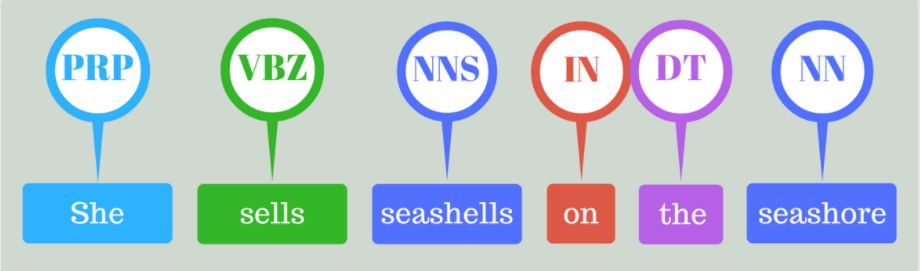
\includegraphics[width=15cm]{img/poslabeling.png}
		\caption{Voorbeeld van PoS-labeling uit het artikel van \textcite{Bilisci2021}.}
		\label{fig:pos-labeling}
	\end{figure}
\end{center}

\medspace

NER-labeling is een techniek om namen van personen, organisaties en locaties te herkennen en te classificeren. Het haalt specifieke informatie uit een tekst, zoals het identificeren van de namen van personen, plaatsen of bedrijven die in nieuwsartikelen, of het extraheren van belangrijke data of getallen uit financiële rapporten, aldus \textcite{Jurafsky2014}. Er zijn vier vormen van NER-labeling, zoals beschreven door \textcite{Li2018}: \textit{dictionary-based}, \textit{rule-based}, \textit{ML-based} en \textit{deep learning-based}. De eerste twee maken gebruik van vooraf gedefinieerde woordenboeken en regels, terwijl de laatste twee gebruik maken van statistische of neurale netwerken om te leren hoe entiteiten te herkennen. Elke vorm maakt gebruik van representaties om entiteiten te modelleren. \textcite{Poel2008} heeft een neurale netwerkmodel onderzocht voor PoS-tagging van Nederlandstalige teksten. Het model behaalde een nauwkeurigheid van 97,88\% voor bekende woorden en 41,67\% voor onbekende woorden en maakte gebruik van de Corpus Gesproken Nederlands (CGN) als trainingsdata. In de verwerking van tekst maken NLP-systemen gebruik van embeddings om woorden numeriek te representeren. Traditionele word embeddings bouwen een woordenschat op zonder de betekenis ervan in context te begrijpen. Contextuele word embeddings begrijpen daarentegen wel de context van een woord \autocite{Eisenstein2019}. 

\section{De verschillende soorten ATS}

Tekstvereenvoudiging kan bijdragen aan het begrijpen van complexe informatie. Zoals onderzocht door \textcite{Siddharthan2014}, zijn er vier soorten transformaties bij ge- automatiseerde tekstvereenvoudiging, waaronder lexicale vereenvoudiging, waarbij eenvoudigere synoniemen de complexe woorden vervangen. Dit heet lexical simplification (LS) of lexicale vereenvoudiging. Bijvoorbeeld, ‘klevend’ kan ‘adhesief’ vervangen. \textcite{Kandula2010} noemt twee manieren om lexicale vereenvoudiging te bewerkstelligen: het vervangen van het woord door een synoniem of het genereren van extra uitleg. De zinsstructuur blijft hetzelfde en de kerninhoud en benadrukking van de tekst blijven behouden. Het doel van lexicale vereenvoudiging is om de moeilijkheidsgraad van de woordenschat in een zin of tekst te verlagen.

\medspace

Diverse onderzoeken hebben aangetoond dat lexicale vereenvoudiging een belangrijke bijdrage kan leveren aan het begrijpen van complexe informatie, en in dit kader wordt de pipeline zoals weergegeven in figuur \ref{img:pipeline-lexical-simplification} vaak gebruikt, bijvoorbeeld in onderzoeken van \textcite{Paetzold2016, Bingel2018, Bulte2018}. Deze pipeline omvat bij de vermelde onderzoeken telkens minstens vier stappen, waarbij de eerste stap \textit{Complex Word Identification} (CWI) is, een gesuperviseerde NLP-taak die moeilijke woorden of \textit{multi-word expressions} (MWE) in een tekst identificeert \autocite{Shardlow2013, Gooding2019}. De LS, waarbij eenvoudigere synoniemen de moeilijkere woorden vervangen, komt na CWI. Hier kunnen ook verklarende beelden of definities komen \autocite{Zeng2005, Kandula2010}. Een goede uitvoering is van cruciaal belang bij CWI, omdat een lage recall van dit component zal resulteren in een uitvoertekst zonder vereenvoudiging van moeilijke woorden zoals opgemerkt door \textcite{Shardlow2013}. Er zijn verschillende manieren geïdentificeerd om substitutiegeneratie uit te voeren, zoals opgesomd in tabel \ref{table:lexical-databases}. Recenter onderzoek, zoals dat van \textcite{Zhou2019}, gebruikt ook een extra \textit{Substitution Ranking} (SR) stap om substituties te rangschikken op basis van relevantie. 

\begin{figure}[H]
	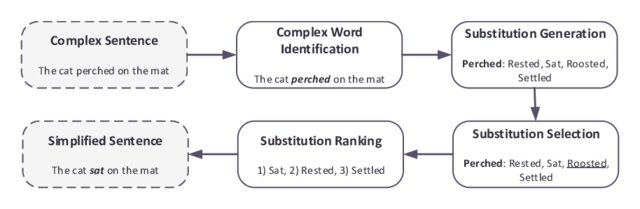
\includegraphics[width=15cm]{img/lexical-simplification-pipeline.png}
	\caption{Een pipeline voor LS volgens \textcite{Althunayyan2021}.}
	\label{img:pipeline-lexical-simplification}
\end{figure}

\begin{center}
\begin{table}[H]
	\begin{tabular}{ | m{7cm} | m{7cm} | } 
		\hline
		\textbf{Databank} & \textbf{Ondersteunde talen} \\
		\hline
		Engels & WordNet \\
		& SWORDS \\
		& LSBert \\
		\hline
		Nederlands & Celex \\
		& NT2Lex \\
		& Cornetto \\
		\hline
		Meertalig (Engels, Duits, Spaans en Portugees) & PHOR-in-One \\
		\hline	
	\end{tabular}
	\caption{Beschikbare Nederlandstalige, Engelstalige en meertalige lexicale databanken anno mei 2023.}
	\label{table:lexical-databases}
\end{table}
\end{center}

\medspace

Syntactische vereenvoudiging is een toepassing om de complexiteit van een zin te verminderen. Het past de grammatica en zinsstructuur van de tekst aan. Dit gebeurt door het combineren van twee zinnen tot één eenvoudigere zin of door de syntax te vereenvoudigen, terwijl de inhouden behouden blijft. Een voorbeeld van zo'n model is ontwikkeld door \textcite{Kandula2010} voor medische informatie. Het model bestaat uit drie modules, die zinnen met meer dan tien woorden vereenvoudigen en eventueel vervangen door kortere zinnen. Het omvat een PoS Tagger, een Grammar Simplifier en een Output Validator als onderdelen van de architectuur.

\medspace

\begin{enumerate}
	\item Ten eerste wordt de PoS Tagger-functie uit het open-source pakket OpenNLP\footnote{https://opennlp.apache.org/} gebruikt.
	\item Vervolgens splitst de \textit{Grammar Simplifier}-module lange zinnen in kortere zinnen door middel van het identificeren van POS-patronen en het toepassen van transformatieregels.
	\item Tot slot controleert de \textit{Output Validator}-module de grammatica en leesbaarheid van de output van de Grammar Simplifier.
\end{enumerate}  

\medspace

Geautomatiseerde tekstvereenvoudiging is geen nieuw concept. Volgens onderzoeken van \textcite{Canning2000, Siddharthan2006} waren de eerste aanpakken op geautomatiseerde tekstvereenvoudiging gebouwd op rule-based modellen. Deze modellen bewerken de syntax door zinnen te splitsen, te verwijderen of de volgorde van de zinnen in een tekst aan te passen. Lexicale vereenvoudiging kwam hier niet aan de pas. Enkel bij recentere onderzoeken van \textcite{Coster2011, Bulte2018} werd het duidelijk hoe lexicale en syntactische vereenvoudiging gecombineerd kon worden.

\medspace

Vroegere onderzoeken tonen aan dat geautomatiseerde tekstvereenvoudiging al geruime tijd bestaat. Zo hebben \textcite{Canning2000} en \textcite{Siddharthan2006} onderzocht dat de eerste methoden gebaseerd waren op \textit{rule-based} modellen die de syntaxis van de tekst bewerken door zinnen te splitsen, te verwijderen of te herschikken. Lexicale vereenvoudiging speelde hierbij geen rol. Enkel de recentere onderzoeken van  Pas bij recentere onderzoeken, zoals die van \textcite{Coster2011, Bulte2018} tonen de mogelijkheid aan om lexicale en syntactische vereenvoudiging te combineren.

\medspace

Om wetenschappelijke artikelen toegankelijker en begrijpelijker te maken, is het van belang om de kernpunten van een artikel op een duidelijke en beknopte manier samen te vatten. Hoewel samenvatten niet gericht is op het vereenvoudigen van de tekst, is het wel een techniek die noodzakelijk is om de semantiek achter een tekst met zo min mogelijk woord- of tekens te kunnen begrijpen. Full-text-search en gepersonaliseerde informatiefiltering benadrukken het belang van deze op maat gemaakte samenvattingen. Een samenvattingssysteem bestaat uit drie fases: analyse van de brontekst, identificatie van de kernpunten en samenvoeging van deze kernpunten tot één overzichtelijke tekst. Het machinaal samenvatten van teksten kan op twee manieren: door extractie en door abstractie \autocite{Hahn2000, Dubay2004}.

\medspace

Het proces van extraherend samenvatten markeert de belangrijkste zinnen in een tekst en herschrijft ze. Dit kan echter leiden tot onsamenhangende uitvoertekst, zoals \textcite{Khan2014} heeft aangetoond. Er zijn verschillende methoden beschikbaar om de kernzinnen te bepalen, zoals woordfrequentie, zinpositie -en gelijkenissen, de \textit{cue}-methode, titels, \textit{proper nouns}, woordgebruik en de afstand tussen \textit{text unit entities}, aldus \textcite{Khan2014}. Verschillende technieken voor het extraherend samenvatten van teksten, waaronder graafgebaseerde methoden, maximal marginal relevance (MMR) en metaheuristiek gebaseerde ES, zijn onderzocht door \textcite{Verma2020} en worden verder beschreven in tabel \ref{table:extractive-summarization}.

\begin{center}
	\begin{table}[H]
	\begin{tabular}{ | m{4cm} | m{12cm} | } 
		\hline
		MMR-gebaseerde ES & Deze traditionele techniek gebruikt de maximaal marginale relevantiescore (MMR) om de relevantie en diversiteit van gemarkeerde zinnen te bepalen. Zorgt ervoor dat de geselecteerde zinnen niet te veel overlappen in inhoud en relevantie. Kan leiden tot betere samenvattingen, maar vereist meer rekenkracht en tijd. \\
		\hline
		Graafgebaseerde ES & Deze techniek vertegenwoordigt een document als een graaf van zinnen en gebruikt algoritmen om de belangrijkste zinnen te bepalen en redundantie te vermijden. Kan zowel voor lange wetenschappelijke artikelen als korte nieuwsartikelen goede resultaten opleveren \autocite{McDonald2007, Lin2010}. \\ 
		\hline
		Metaheuristiek-gebaseerde ES & Deze techniek maakt gebruik van optimalisatie-algoritmen zoals genetische algoritmen en zwermoptimalisatie om de belangrijkste zinnen in een tekst te vinden \autocite{Premjith2015, Verma2020}. Evaluatiefunctie kan in een lokaal optimum vastlopen afhankelijk van de gebruikte criteria. \autocite{Rani2021}. \\
		\hline
	\end{tabular}
	\caption{De drie manieren om extraherende samenvatting mogelijk te maken volgens \textcite{Verma2020}.}
	\label{table:extractive-summarization}
	\end{table}
\end{center}

\medspace

Vooroordelen of een \textit{bias} kan de extraherende samenvatting van nieuwsartikelen beïnvloeden, zo blijkt uit experimenten uitgevoerd door \textcite{McKeown1999}. Deze vorm van samenvatten neemt de zinnen over zoals ze zijn. \textcite{Hahn2000} bouwde verder op deze experimenten door het combineren van \textit{knowledge-rich} en \textit{knowledge-poor} methoden, wat resulteerde in significante verbeteringen. Bij het extraherend samenvatten is het van belang om de meest relevante tekstgedeeltes te selecteren, meestal in de vorm van zinnen. Om de lexicale en statistische relevantie van een zin te kunnen bepalen, noemen \textcite{Hahn2000} twee methoden:

\begin{itemize}
	\item Het lineaire gewichtsmodel, waarbij elke teksteenheid wordt gewogen op basis van factoren zoals de positie van de zin en het aantal keren dat deze voorkomt.
	\item Het gewichtsmodel op basis van de statistische relevantie van een eenheid, waarbij rekening wordt gehouden met de aanwezigheid van woorden in titels.
\end{itemize}

\medspace

Om de nauwkeurigheid van modellen te verbeteren, ontwikkelden \textcite{Nallapati2017} \textit{SummaRuNNer}. Dit model kan teksten extraherend samenvatten door een neuraal netwerk. Zo gebruikt het \textit{PyTorch} en bestaat het uit drie modellen: een recurrent neuraal netwerk, een convolutioneel recurrent neuraal netwerk en een \textit{hiërarchical attention network}.

\medspace

Extraherende samenvattingen kunnen leiden tot een onsamenhangende tekst. Abstraherende samenvatting kan een oplossing bieden, omdat het rekening houdt met de samenhang van een tekst. Onderzoek van \textcite{Gupta2019} wijst twee benaderingen voor abstraherende samenvatting: semantisch-gebaseerd en structuurgebaseerd. De structuurgebaseerde methode gebruikt regels om belangrijke informatie in de tekst te vinden, maar dit kan leiden tot samengevatte zinnen van lage taalkundige kwaliteit en grammaticale fouten. De semantisch-gebaseerde benadering daarentegen gebruikt de betekenis van de tekst om korte en duidelijke samenvattingen te maken met minder redundante zinnen en een betere taalkundige kwaliteit. Een extra parsingfase kan van pas komen volgens de onderzoeken. Onderzoeken van \textcite{Suleiman2020, Cao2022} wijzen \textit{deep learning}-methoden uit om automatisch abstraherende samenvattingen te genereren. Zo kunnen RNN's, CNN's en Seq2Seq dienen om abstraherende samenvatting mogelijk te maken. 

\medspace

Ontwikkelaars moeten een andere aanpak gebruiken wanneer zij een systeem willen ontwikkelen voor \textit{long text summarization} of LTS, zoals bij boeken of wetenschappelijke tijdschriften. Zo kan het opsplitsen van de tekst leiden tot het breken van samenhangende paragrafen. Dat kan later resulteren in redundante tekst in het samengevatte document. Zo raadden onderzoeken van \textcite{Hsu2018, Huang2019} aan om zowel extraherend als abstraherende samenvatting toe te passen. Om deze reden zou een \textit{hybrid summarization pipeline} twee fasen moeten bevatten: een inhoudselectiefase waarbij het systeem kernzinnen extraheert, gevolgd door een parafraserende fase.

\medspace

Daarnaast moeten ontwikkelaars ook rekening houden met de doelgroep wanneer zij een systeem of model uitkiezen voor tekstvereenvoudiging of samenvatting. Zo moeten ontwikkelaars rekening houden met de individuele behoeften en uitdagingen van elke scholier, volgens \textcite{Gooding2022}. Dyslexie kan zich namelijk op verschillende manieren uiten bij verschillende scholieren, waarbij bijkomende symptomen niet altijd van invloed zijn op de spellingprestaties van een scholier. Om deze reden is het belangrijk om een toepassing te ontwerpen die rekening houdt met de diversiteit van dyslexie.

\section{Beschikbare tools en taalmodellen}
\label{sec:beschikbare-tools-en-taalmodellen}

Het kan moeilijk zijn voor scholieren met dyslexie om goed te lezen en te schrijven. Gelukkig zijn er verschillende softwareprogramma's en tools beschikbaar om hen te ondersteunen. Deze sectie gaat in op de nationale en internationale software die specifiek is ontworpen voor scholieren met dyslexie om hen te helpen bij het lezen van teksten.  Er zal voornamelijk worden gekeken naar beschikbare software in Vlaamse middelbare scholen, chatbots zoals Bing Chat en ChatGPT, en software die speciaal is ontwikkeld om dyslexie bij het lezen te ondersteunen. Deze sectie beantwoordt de volgende deelvraag: 

\begin{itemize}
	\item Welke toepassingen, tools en modellen zijn er beschikbaar om Nederlandstalige geautomatiseerde tekstvereenvoudiging met AI mogelijk te maken?
\end{itemize}

\medspace

Scholieren met dyslexie krijgen in het middelbaar onderwijs enkel ondersteuning in de vorm van voorleessoftware \autocite{DeCraemer2018, OnderwijsVlaanderen2023}. Het ministerie van Onderwijs in Vlaanderen biedt licenties aan voor verschillende softwarepakketten zoals SprintPlus, Kurzweil3000, Alinea Suite, IntoWords en TextAid, die scholieren kunnen gebruiken om zinnen te markeren en deze vervolgens samen te vatten. Het samenvatten gebeurt echter op een manier waarbij de zinnen lexicaal en syntactisch identiek blijven. Helaas bieden deze softwarepakketten geen functie voor het vereenvoudigen van teksten. Volgens \textcite{Tops2018} is het belangrijk om deze software zo vroeg mogelijk in de schoolcarrière te introduceren, zodat scholieren er snel vertrouwd mee raken en het optimaal kunnen gebruiken in verdere studies. Hoewel \textcite{Tops2018} de handige aspecten van deze software benadrukt, is het te laat om deze software pas in het hoger onderwijs te introduceren.

\medspace

Momenteel hebben scholieren met dyslexie in het middelbaar onderwijs beperkte tekstvereenvoudigingsfunctionaliteiten in de bestaande voorleessoftware. Dit onderstreept de noodzaak aan nieuwe erkende tools die tekstvereenvoudiging in het onderwijs mogelijk maken. Tools zoals Simplish en Rewordify kunnen een oplossing bieden. Hoewel Simplish oorspronkelijk Engelstalig is, is het inmiddels mogelijk om een vereenvoudigde tekst te genereren van Nederlandstalige teksten, al is deze functionaliteit betalend voor niet-Engelstalige teksten. Rewordify is enkel in staat om Engelstalige teksten te vereenvoudigen. Er zijn echter maar weinig proof-of-concepts beschikbaar en de taalmodellen waarop deze applicaties werken zijn niet gekend om deze tools te kunnen repliceren. Bovendien zijn er geen API's beschikbaar om mee te werken. 

\medspace

Voor samenvatting zijn er echter meer tools beschikbaar. Enkele voorbeelden hiervan zijn Resoomer, Paraphraser, Editpad, Scribbr en Quillbot. Al zijn er onderzoeken over geautomatiseerde lexicale en syntactische vereenvoudiging voor scholieren met dyslexie, het aantal onderzoeken over samenvatten voor deze doelgroep is schaars. Zoals eerder aangehaald is er wel onderzoek gedaan naar de verschillende manieren om een tekst samen te vatten, maar er is geen toepassing of onderzoek dat dit concreet uitwerkt. \textcite{Sanja2021} wijzen erop dat toepassingen voor tekstvereenvoudiging regelmatig als \textit{showcase} van de technologie ontwikkeld worden en zelden tot weinig rekening houden met gepersonaliseerde samenvatting om zo rekening te houden met de verschillende noden.

\medspace

Er zijn weinig toepassingen beschikbaar om wetenschappelijke artikelen te vereenvoudigen, maar er bestaan gratis en betalende toepassingen. Zo reiken SciSpace\footnote{https://typeset.io/} en Scholarcy ATS specifiek voor wetenschappelijke artikelen aan.  en Scholarcy\footnote{https://www.scholarcy.com/}. Hero vloeide verder uit het onderzoek van \textcite{Bingel2018}, waarbij de onderzoekers een toepassing voor gepersonaliseerde ATS voor kinderen met dyslexie ontwikkelden. Hoewel Hero een oplossing aanreikt, slaagt de toepassing er niet in om wetenschappelijke artikelen te vereenvoudigen. Wel kunnen scholieren deze browserextensie gebruiken voor selecte Engelstalige nieuwssites. Tabel \ref{table:overview-tools} geeft een overzicht van prevalente tools die momenteel tekstvereenvoudiging aanbieden.

\begin{center}
	\begin{table}[H]
		\begin{tabular}{ | m{4cm} | m{12cm} | } 
		\hline
		\textbf{Tool} & Algemene functionaliteit \\
		\hline
		Sprintplus & \\
		Kurzweil3000 & \\
		Alinea Suite & Voorleessoftware met ondersteuningsmogelijkheden voor moeilijke woordenschat \\
		IntoWords & \\
		TextAid & \\
		\hline
		Resoomer &  \\
		Paraphraser & \\
		Editpad & Samenvattingstool \\
		Scribbr & \\
		Quillbot & \\
		\hline
		SciSpace & Samenvattingstool specifiek voor wetenschappelijke artikelen. \\
		Scholarcy & \\
		\hline
		Simplish & Tool voor tekstvereenvoudiging met bijhorende analyse\\
		Rewordify & \\
		\hline
		\end{tabular}
	\caption{Overzicht van gekende voorleessoftware, tekstvereenvoudigings- en samenvattingstools die intuïtief zijn ontwikkeld voor de eindgebruiker (leerkracht of scholier).}
	\label{table:overview-tools}
	\end{table}
\end{center}

\medspace

Ontwikkelaars kunnen ook zelf aan de slag gaan. Zo beschikt Huggingface een breed scala aan API's en tools die gemakkelijk te downloaden en trainen zijn voor \textit{pretrained} modellen voor veelvoorkomende NLP-taken, zoals \textit{text classification}, taalmodellering en samenvatting. Tekstvereenvoudiging is in mindere mate aanwezig. Verder kunnen ontwikkelaars deze modellen \textit{finetunen} op specifieke datasets om modellen te bouwen voor gepersonaliseerde NLP-taken. Ten slotte geeft tabel \ref{table:huggingface-models} taalmodellen van HuggingFace met hun respectievelijke casus.

\medspace

\begin{center}
	\begin{table}[H]
	\begin{tabular}{ | m{4cm} | m{12cm} | } 
		\hline
		\textbf{Taalmodel} & Specifieke casus \\ \hline
		Google Pegasus & Samenvattingstaken voor kort tot middelgrote documenten. \\
		\hline
		Longformer Encoder-Decoder & Samenvatting van lange wetenschappelijke artikelen \\
		\hline
		Haining Scientific Abstract Simplification\footnote{https://huggingface.co/haining/scientific\_abstract\_simplification} & Het lexicaal vereenvoudigen van wetenschappelijke artikelen. \\
		\hline
		BART Large Scientific Summarisation\footnote{https://huggingface.co/sambydlo/bart-large-scientific-lay-summarisation} & Het samenvatten van wetenschappelijke artikelen. \\
		\hline
		T5 finetuned text simplification model\footnote{https://huggingface.co/husseinMoh/t5-small-finetuned-text-simplification} & Tekstvereenvoudiging voor algemeen gebruik. \\
		\hline
		Keep It Simple\footnote{https://huggingface.co/philippelaban/keep\_it\_simple} & Ongesuperviseerde tekstvereenvoudiging met ATS. \\
		\hline
	\end{tabular}
		\caption{HuggingFace beschikbare en ge-finetunede taalmodellen.}
		\label{table:huggingface-models}
	\end{table}
\end{center}

\medspace

Dankzij de sterke evolutie in data en AI, kon de grootte van deze taalmodellen sterk vergroten. Zo is GPT-3 een opkomend \textit{Large Language Model} of LLM. OpenAI ontwikkelde dit taalmodel en pastte daarvoor een tweestapsleerparadigma toe \autocite{Radford2019, Li2022}. 

\begin{itemize}
	\item Allereerst komt er een ongesuperviseerde training aan bod met een \textit{language modelleing goal}. Ontwikkelaars trainden dit model op niet-gecategoriseerde data van het internet met datasets zoals Common Crawl, WebText2, Books1, Books2 en Wikipedia.
	\item Tenslotte finetunen de ontwikkelaars dit verder. Om een correcte respons van het model te krijgen, passen de ontwikkelaars \textit{reinforcement learning} toe.
\end{itemize}

GPT-3 beschikt over meerdere versies, waaronder GPT-3.5 die als engine dient voor ChatGPT. Omdat onbegrijpelijke en ontoegankelijke zinsstructuren niet alleen voor leken, maar ook voor vakexperten een obstakel vormen, is het belangrijk om te benadrukken dat GPT-3.5 gericht is op conversationele doeleinden, terwijl GPT-3 in het algemeen bedoeld is om met hoogstens één prompt te werken \autocite{McNutt2014, Hubbard2017}.

\medspace

Volgens \textcite{Gooding2022} kan een toepassing zoals ChatGPT de leesbaarheid van een tekst op twee manieren bevorderen. Ten eerste kan het unieke versies van een tekstvereenvoudiging leveren, waardoor de gebruiker uit meerdere vereenvoudigingen kan kiezen. Figuur \ref{img:different-versions-gooding} illustreert dit verder.  Zo geeft Gooding aan dat het taalmodel de invoertekst op meerdere manieren kan vereenvoudigen. Verder bespreekt Gooding in figuur \ref{img:evaluation-gooding} de prompt-gebaseerde evaluatiemanier van GPT-3. Het model kan de verschillen tussen de gegenereerde teksten begrijpen en de gebruiker feedback geven. In figuur \ref{img:simplification-gooding} laat Gooding zien hoe het model lexicale, conceptuele en syntactische vereenvoudiging kan toepassen op een paragraaf uit een boek van de Russische schrijver Dostoevsky.

\begin{figure}[H]
	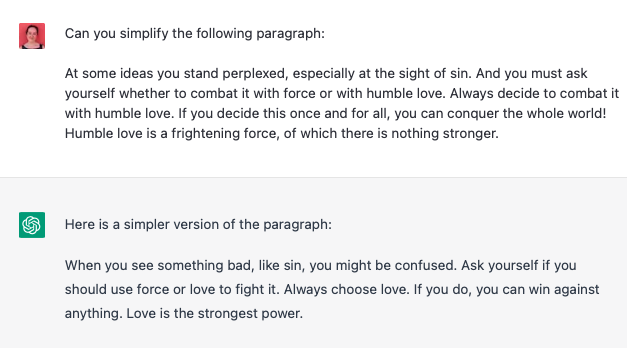
\includegraphics[width=\linewidth]{img/chatgpt-example-simplification-gooding.png}
	\caption{Afbeelding van Gooding 2022}
	\label{img:simplification-gooding}
\end{figure}

\begin{figure}[H]
	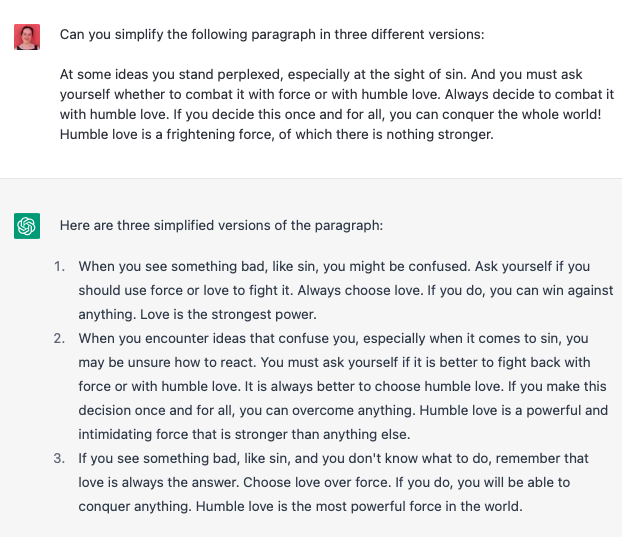
\includegraphics[width=\linewidth]{img/chatgpt-example-different-versions-gooding.png}
	\caption{Afbeelding van Gooding 2022}
	\label{img:different-versions-gooding}
\end{figure}

\begin{figure}[H]
	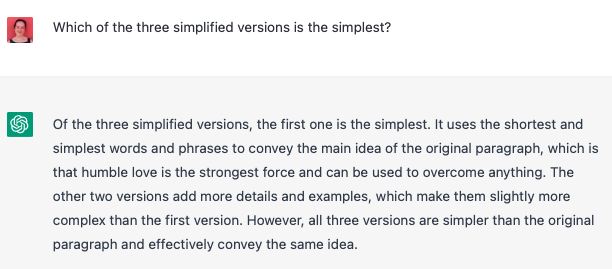
\includegraphics[width=\linewidth]{img/chatgpt-example-evaluation-gooding.png}
	\caption{Afbeelding van Gooding 2022.}
	\label{img:evaluation-gooding}
\end{figure}

OpenAI reikt documentatie aan voor het GPT-3 taalmodel. Daarin vermelden ze vier \textit{engines}, namelijk Davinci, Curie, Babbage en Ada. In maart 2023 kwam daar een vijfde engine bij, namelijk GPT-3 Turbo die fungeert als achterliggende engine voor Chat-GPT. Davinci-003 is het meest geavanceerde model, geschikt voor taken zoals het schrijven van essays en het genereren van code, en levert de meest menselijke antwoorden. Curie is goed in nuance, maar minder menselijk dan Davinci, terwijl Ada en Babbage minder krachtig zijn en beter geschikt zijn voor eenvoudige taken zoals het aanvullen van tekst en sentimentanalyse \autocite{Brockman2023}. Deze engines gebruiken dezelfde set hyperparameters, die ontwikkelaars kunnen aanpassen. Tabel \ref{table:gpt-3-parameters} somt deze parameters verder op.

\medspace

\begin{center}
	\begin{table}[H]
	\begin{tabular}{ m{3cm} | m{7cm} | m{5cm} }
		\hline
		\textbf{Parameter} & \textbf{Omschrijving} & \textbf{Mogelijke waarden} \\
		\hline
		model & De GPT-3 engine die ontwikkelaars kunnen gebruiken. & davinci, curie, babbage, ada, text-davinci-002, text-curie-001, text-babbage-001, text-ada-001, davinci-codex \\
		\hline
		temperature & De gulzigheid van het generatief model. Een lagere waarde kan voorspelbare tekst teruggeven. Hogere waarden daarentegen kunnen onverwachtse tekst teruggeven, wat beter werkt bij creatieve toepassingen. & Een kommagetal tussen 0 en 1. \\
		\hline
		max tokens & Het maximaal aantal tokens (woorden of subwoorden) dat het generatief model kan teruggeven. & Een getal tussen 1 and 2048. \\
		\hline
		top-p & Vergelijkbaar met temperature, maar deze waarde onderhoudt de \textit{probability distribution} voor \textit{common tokens}. Hoe lager de waarde, hoe hoger de woordfrequentie van de gegenereerde tekst. Toepassingen gericht op nauwkeurigheid maken beter gebruik van hoge waarden. & Een kommagetal tussen 0 en 1. \\
		\hline
		stop & Een tekstwaarde (woord/symbool) tot waar het model zal genereren. & String-waarden \\
		\hline
		presence penalty & Factor die bepaalt hoe regelmatig woorden voorkomen & Kommagetallen tussen 0 en 1 \\
		\hline
	\end{tabular}
		\caption{Tabel met alle GPT-3 parameters.}
		\label{table:gpt-3-parameters}
	\end{table}
\end{center}

Hoewel onderzoeken rond GPT-3 nog volop in ontwikkeling zijn, bestaan er vergelijkende onderzoeken naar de mogelijkheden van dit LLM. Onderzoek van \textcite{Binz2023} wijst uit dat de mean-regret score kan dienen als maatstaf om de menselijkheid van antwoorden te beoordelen. Deze studie wees verder uit dat deze modellen capabel zijn om menselijke antwoorden te produceren, zoals geïllustreerd in figuur \ref{img:mean-regret-chatgpt}. Uit het experiment van \textcite{Goyal2022} blijkt dat \textit{zero-shot} samenvattingen met GPT-3 beter presteren dan gefinetunede modellen. \autocite{Li2022} benadrukt dat GPT-3 overkill is voor taken zoals sentimentanalyse -of classificatie. Daarvoor halen de onderzoekers aan om een kleinschaliger taalmodel te gebruiken. Deze taalmodellen beschikken ook over een grotere ecologische voetafdruk, waarvoor onderzoeken van \textcite{Strubell2019, Simon2021} deze praktijk ook afraden. Ten slotte bestaan er al enkele tools die gebruikmaken van de GPT-3 API, waaronder Jasper AI en ChatSonic zoals aangehaald in het onderzoek van \textcite{Mottesi2023}. Experten zoals \textcite{Roose2023, Garg2022} halen het GPT-3 model en ChatGPT aan als de toekomst voor gepersonaliseerde en adaptieve uitleg aan scholieren. Bing Chat biedt een extra dat revolutionair kan zijn bij het opzoeken van uitleg voor zoektermen, zonder het verlies aan bronvermelding. Dankzij de personalisering van de prompts biedt GPT-3 mogelijkheden aan voor toepassingen in het onderwijs, aldus \textcite{Roose2023, Garg2022}.

\begin{figure}[H]
	\begin{center}
		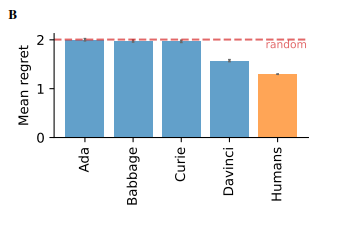
\includegraphics[width=\linewidth]{img/chatgpt-engines-mean-regret.png}
		\caption{Een experiment op de \textit{mean-regret} van GPT-3 engines uit \textcite{Binz2023}.}
		\label{img:mean-regret-chatgpt}
	\end{center}
\end{figure}

\medspace


Met neurale netwerken kan het taalmodel patronen in de input herkennen. Deze patronen dienen om voorspellingen te maken over de output \autocite{Liu2020}. Via prompts hebben mensen toegang tot krachtige taalmodellen, zoals GPT-3 of BERT \autocite{McFarland2023, Harwell2023}. Figuur \ref{img:prompt-engineering} illustreert de werking van deze vaardigheid. Onderzoek van \textcite{Liu2020} benadrukt het belang van goed opgestelde prompts. Hiervoor kunnen eindgebruikers de technieken in tabel \ref{table:techniques-for-good-prompts}. Zo moeten deze werk kunnen produceren op maat van het doel. Zo benadrukt de onderzoeker dat een prompt concreet moet zijn. Bij het opstellen van een prompt voor een zoekopdracht is het cruciaal om voldoende parameters op te nemen om te voorkomen dat het model te algemeen blijft en afwijkt van de intentie van de gebruiker. Effectieve prompt engineering voor AI leidt tot hoogwaardige trainingsgegevens, waardoor het AI-model nauwkeurige voorspellingen en beslissingen kan maken \autocite{Liu2020}.

\begin{table}
	\begin{tabular}{| m{5cm} | m{5cm} | }
		\hline
		\textbf{Prompttechniek} & \textbf{Bron} \\ \hline
		Duidelijke scope & \autocite{McFarland2023} \\ \hline
		Specifieke sleutelwoorden & \autocite{McFarland2023} \\ \hline
		De context waarin de vraag zich afspeelt. & \autocite{McFarland2023} \\ \hline
		Gepersonaliseerde keuzes & \autocite{McFarland2023} \\ \hline
	\end{tabular}
	\caption{Technieken voor concrete en goed opgestelde prompts.}
	\label{table:techniques-for-good-prompts}
\end{table}

\begin{figure}[H]
	\begin{center}
		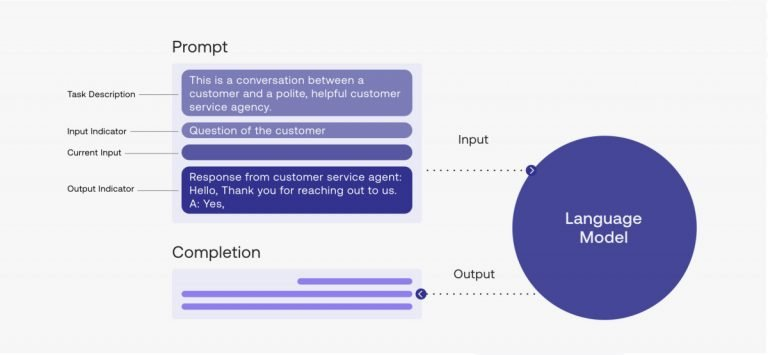
\includegraphics[width=\linewidth]{img/prompt-engineering-medium.png}
	\end{center}
	\caption{De werking van \textit{prompt engineering} volgens \textcite{McFarland2023}}
	\label{img:prompt-engineering}
\end{figure}

Om prompts te kunnen hergebruiken, bouwden ontwikkelaars \textit{prompt patterns} op. Deze patronen bieden herbruikbare oplossingen voor veelvoorkomende problemen in een bepaalde context, vooral bij de interactie met LLM's. \textcite{White2023} benoemt vier \textit{prompt patterns}:

\begin{itemize}
	\item	\textit{Intent prompts} waarbij een LLM een instructie krijgt met een specfiek verwacht antwoord.
	\item	\textit{Restriction prompts} die het antwoord van een LLM inperkt. Deze pattern is noodzakelijk om een LLM binnen de lijnen te houden.
	\item 	\textit{Contextualization prompts} verzekeren dat de output van een LLM relevant is. De prompt bevat de context.
	\item	\textit{Expansion/reduction prompts} genereren een beknopte output met voldoende details. 
\end{itemize}

\medspace

BERT is een meertalige LLM die gebruikmaakt van \textit{contextual word embeddings}. Onderzoekers trainden het model op 110 miljoen parameters uit 104 verschillende talen, waaronder Nederlands. Voor de Nederlandse taal zijn er twee varianten van BERT beschikbaar: RobBERT en BERTje. GPT-3 en BERT beschikken over een verschillende architectuur. Zo is volgens \textcite{Mottesi2023} GPT-3 een autoregressief model dat alleen rekening houdt met de linkercontext bij het voorspellen of genereren van tekst. BERT daarentegen is een bidirectioneel model, waarbij het model zowel de linker- als de rechtercontext in overweging neemt. De bidirectionele werking van BERT is geschikt voor sentimentanalyse, waarbij begrip van de volledige zincontext noodzakelijk is. Omdat GPT-3 toegang heeft tot meer informatie (45TB) dan BERT (3TB), kan dit een voordeel bieden tijdens taalbewerkingen zoals vereenvoudigen, parafraseren of vertalen. Ten slotte verschillen de LLM's ook qua grootte. Hoewel beide modellen erg groot zijn, is GPT-3 aanzienlijk groter dan BERT, mede door de uitgebreide trainingsdatasetgrootte \autocite{Brown2020}. Er is echter een nieuw generatief taalmodel genaamd LLaMa, dat sterker is dan GPT-3 en vergelijkbare modellen, terwijl het slechts tien keer minder parameters gebruikt. Helaas is LLaMa momenteel nog niet beschikbaar als online webtoepassing of API \autocite{Hern2023, Touvron2023}. Figuur \ref{img:graph-language-models} toont de evolutie van \textit{pre-trained} taalmodellen. Zo volgt de LLM-performantie ten opzichte van het aantal parameters van een LLM een lineaire functie.

\begin{figure}[H]
	\begin{center}
		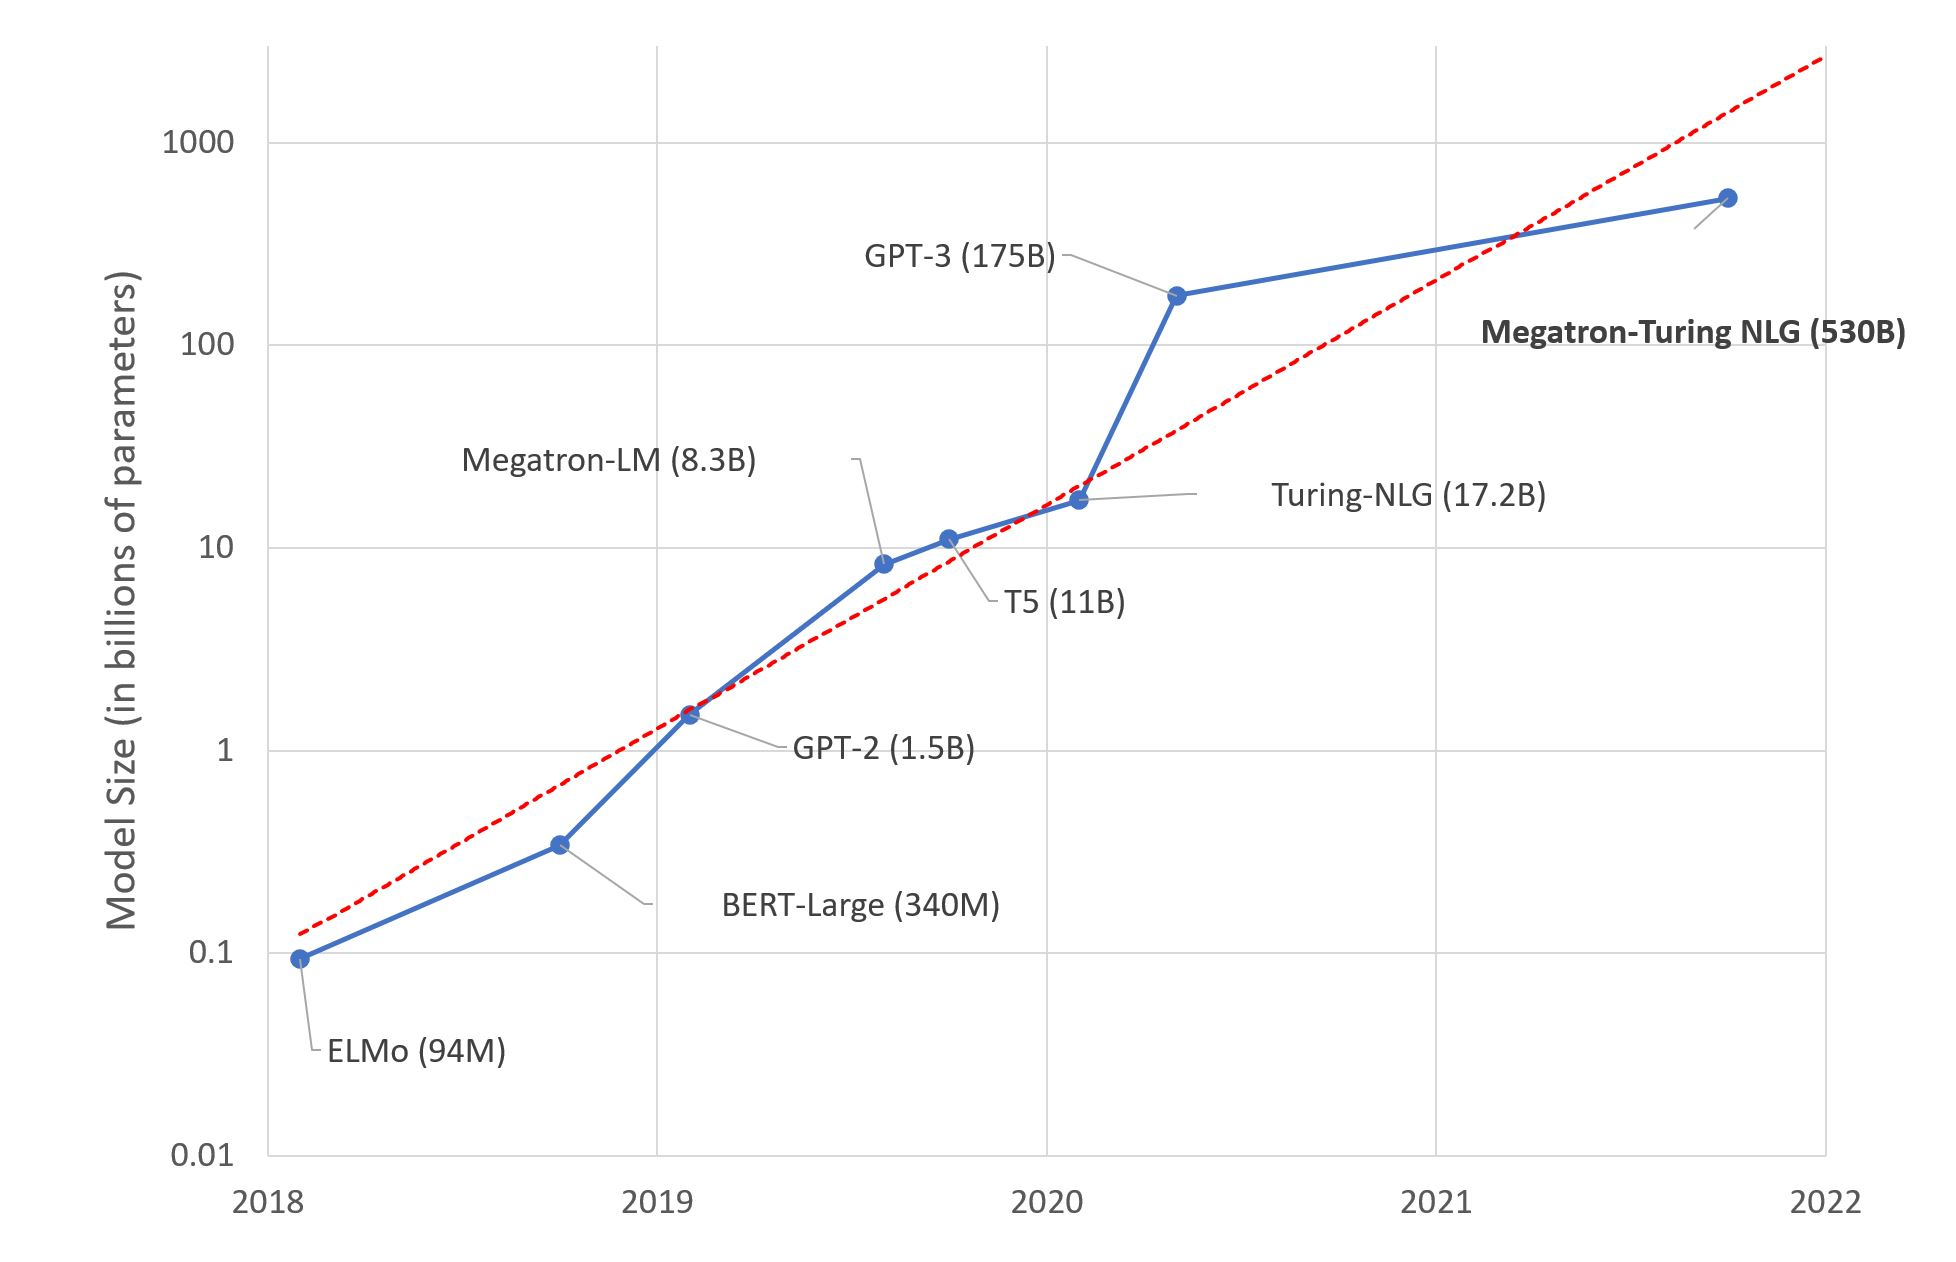
\includegraphics[width=\linewidth]{img/graph-language-models.png}
		\caption{De evolutie van LLM's \autocite{Simon2021}}
		\label{img:graph-language-models}
	\end{center}
\end{figure}

Microsoft en OpenAI werken nauw samen. Zo gebruikt Bing Chat ook het GPT-3 taalmodel. Met de Prometheus-technologie kan deze chatbot verder bouwen en verwijzingen bieden naar andere websites \autocite{Ribas2023}. Zo maakt Bing Chat verwijzingen naar bestaande online documenten dankzij de Bing index-, ranking- en antwoordresultaten. Prometheus combineert dit met het redeneervermogen van OpenAI’s GPT-modellen. Via de \textit{Bing Orchestrator} genereert Prometheus iteratief een set \textit{internal queries} om zo binnen de gegeven gesprekscontext nauwkeurige antwoorden op gebruikersvragen te bieden \autocite{Ribas2023}. Bing Chat is beschikbaar als webpagina en browserextensie voor Microsoft Edge. Het gebruik van extraherende en abstraherende samenvattingen maakt de chatbot interessant, al bestaat er nog te weinig onderzoek naar de credibiliteit en correctheid van de verstrekte verwijzingen. Daarnaast beschikt Bing Chat niet over een API, waardoor ontwikkelaars geen commandlinetoepassingen met deze technologie kunnen maken.

\section{De valkuilen bij AI en NLP.}

AI en ML zijn volop in groei. NLP gebruikt AI en ML om menselijke taal te verwerken, terwijl NLU deze technologieën gebruikt om menselijke taal te begrijpen. Hoewel deze technologieën veelbelovend zijn, moeten AI-ontwikkelaars rekening houden met veelvoorkomende en genegligeerde uitdagingen en valkuilen \autocite{Sciforce2020, Roldos2020, Khurana2022}. Deze sectie beantwoordt de volgende onderzoeksvraag: 

\begin{itemize}
	\item Met welke valkuilen bij taalverwerking met AI moeten ontwikkelaars rekening houden?
\end{itemize}

\medspace

Het ontwikkelen van NLP- en NLU-toepassingen is duur en vormt een obstakel voor veel IT-professionals vanwege factoren zoals het gebrek aan NLP-expertise, de kwaliteit en kwantiteit van data, de integratie en deployment van modellen en de transparantie van modellen \autocite{IBM2022}. Bij de ontwikkeling en finetuning van een NLP-toepassing met AI verkiezen software-ontwikkelaars \textit{black-box} modellen. Hoewel het verschil in nauwkeurigheid minimaal is, wordt de afweging gemaakt op basis van de transparantie van het model. Na een transformatie wordt niet aangegeven waarom specifieke transformaties zijn uitgevoerd, zoals het vervangen van een woord door een eenvoudiger synoniem. \textit{White-box} taalmodellen zijn schaars \autocite{Punardeep2020}.

\medspace 

Sequence labeling kan worden bemoeilijkt door homoniemen, zoals beschreven in onderzoek door \textcite{Roldos2020}. Een voorbeeld hiervan is het woord 'bank', dat voor de machine niet duidelijk aangeeft of het gaat om de financiële instelling of het meubelstuk. Methoden zoals Word Sense Disambiguation (WSD), PoS-tagging en contextual embeddings kunnen de betekenis van woorden bepalen op basis van de context \autocite{Eisenstein2019, Liu2020}. Het verbeteren van NLP-systemen met synoniemen en antoniemen kan worden bereikt door het gebruik van candidate generation en synonym detection, terwijl meertalige transformers zoals BERT een oplossing bieden voor de beperkte toepassingen in andere talen dan het Engels \autocite{Dandekar2016, Roldos2020}.

\medspace

Verschillende studies hebben aangetoond dat tekstvereenvoudiging bedoeld is om gelijke kansen te bieden aan iedereen. Bij het ontwikkelen van adaptieve tekstvereenvoudigingstoepassingen is het echter belangrijk om ethische overwegingen en bewustzijn van de behoeften van de eindgebruiker in acht te nemen, zoals beschreven in onderzoeken van \textcite{Niemeijer2010}, \textcite{Xu2015}, en \textcite{Gooding2022}. Om de eindgebruiker meer controle te geven, moet deze de keuze hebben om te kiezen welke delen van de tekst vereenvoudigd moeten worden, wat kan worden bereikt door synoniemen te gebruiken of zinnen te markeren die moeilijk te begrijpen zijn.

\medspace

Hoewel iedereen kan converseren met een chatbot, vereist het verkrijgen van gepaste en verwachte antwoorden een doordachte input. Onnauwkeurige prompts of een gebrek aan trainingsdata kunnen leiden tot onjuiste output. Door het gebruik van conditionele expressies of het finetunen van hyperparameters kan echter de betrouwbaarheid van de antwoorden worden vergroot \autocite{Miszczak2023, Jiang2023}.

\medspace

Het beoordelen van vereenvoudigde teksten vereist de nodige opvolging van ontwikkelaars in vergelijking met andere ML- of NLP-taken. Evaluatiemetrieken zoals ROUGE en BLEU zijn beperkt omdat ze geen rekening houden met de semantiek tussen een referentietekst en een vereenvoudigde of samengevatte tekst. Om dit probleem op te lossen, beveelt \textcite{Fabbri2020} aan dat ontwikkelaars menselijke evaluatie inschakelen om de vereenvoudigde tekst van een taalmodel te beoordelen. De onderzoekers dringen aan op verdere studie naar nieuwe standaarden en beste praktijken voor betrouwbare menselijke beoordeling. Bovendien moeten de doelgroepen voor wie de tekst wordt vereenvoudigd, nauw betrokken worden bij het proces \autocite{Iskender2021}. Tabel \ref{table:summary-hurdles} somt de aangehaalde struikelblokken bij de ontwikkeling van NLP-toepassingen op.

\medspace

\begin{center}
	\begin{table}[H]
	\begin{tabular}{ m{4cm} | m{10cm} | }
		\hline
		\textbf{Probleem} & \textbf{Oplossing} \\
		\hline
		Dure ontwikkeling en onderhoud van taalmodellen & Voorkeur voor black-box modellen bij ontwikkeling en finetuning. API's kunnen als alternatief dienen op zelf-gehoste taalmodellen. \\
		\hline
		Homoniemen kunnen sequence labeling bemoeilijken & Word Sense Disambiguation, PoS-tagging en contextual embeddings. \\
		\hline
		Paternalisme & Ontwikkeling van gepersonaliseerde tekstvereenvoudigingstoepassingen moeten de eindgebruiker meer controle geven, zoals het kiezen welke delen van de tekst vereenvoudigd moeten worden, het gebruik van synoniemen of het markeren van zinnen die moeilijk te begrijpen zijn. \\
		\hline
		Onnauwkeurige prompts & Gebruik van conditionele expressies bij prompts of one-shot summary uitvoeren. \\
		\hline
		Onnauwkeurige evaluatie van tekstvereenvoudiging & Menselijke evaluatie toepassen of gebruik maken van ROUGE-L metrieken die wel de semantiek in achting nemen. 
		\hline
	\end{tabular}
	\caption{Samenvattend schema met vaak voorkomende struikelblokken bij NLP-toepassingen.}
	\label{table:summary-hurdles}
	\end{table}
\end{center}

\section{Conclusie}

% 	\item Welke specifieke noden hebben scholieren met dyslexie van de derde graad middelbaar onderwijs bij het begrijpen van complexere teksten?
%   \item Wat zijn de specifieke kenmerken van wetenschappelijke artikelen?

Begrijpend lezen is voor scholieren met dyslexie in de derde graad van het middelbaar niet enkel moeizaam, maar gaat verder dan dat. Deze scholieren kunnen moeite ondervinden bij het decoderen en automatiseren van woordherkenning. MTS en aangepaste opmaakopties bieden bewezen voordelen voor scholieren met dyslexie. Zo kunnen de MTS-technieken, besproken in \ref{table:benefits-mts} dienen als aftoetscriteria. Daarnaast neemt de leesbaarheid van wetenschappelijke artikelen neemt af. Het gebruik van vakjargon, ingewikkelde woordenschat en moeizame syntax sluiten een algemeen publiek uit en maken het enkel mogelijk voor wetenschappelijk geletterden om deze artikelen te lezen.

% 

Een uniform formaat en de evolutie van LLM's bieden kansen voor gepersonaliseerde ATS aan, waarbij experts tactieken hebben ontwikkeld om teksten te vereenvoudigen op maat voor scholieren met dyslexie. Gerichte menselijke vergelijkingen en leesbaarheidsformules dienen als evaluatie voor de vereenvoudigde teksten door ATS.

Er zijn taalmodellen beschikbaar in de vorm van API's of open-source software die deze transformaties kunnen uitvoeren. De overheid leent voornamelijk leessoftware uit, maar LLM's bieden mogelijkheden aan voor gepersonaliseerde ATS. Ontwikkelaars moeten zich echter bewust zijn van het feit dat andere taalmodellen zoals BERT voor taken zoals semantische analyse soms betere resultaten leveren met minder rekenkracht.